\documentclass[English, 11pt, twoside, authoryear]{article}
\setlength{\columnsep}{20pt} % column separation width
%\usepackage{txfonts} %font package that is more up to dater than times
\usepackage{natbib}
\usepackage{graphicx}
%\usepackage{wrapfig}
\usepackage{subfigure} %% make it possible to include more than one captioned figure/table in a single float
\usepackage[dvipsnames]{xcolor}
%\usepackage{multicol}
\usepackage{multirow}
%\usepackage{booktabs}
\usepackage{topcapt} % top caption for tables
%\usepackage{a4wide} % makes the text on a page wider
\usepackage{booktabs} % for much better looking tables
\usepackage{paralist} % very flexible & customisable lists (eg. enumerate/itemize, etc.)
\usepackage{verbatim} % adds environment for commenting out blocks of text (\begin{comment} ... \end{comment}) & for better verbatim

%% ---- package for formatting code with line numbers
\usepackage{listings}
\lstset{
backgroundcolor = \color{yellow},
frame = single,
breaklines = false,
firstnumber = 1,
numbers = left,
language = Bash,
basicstyle = \ttfamily,
showstringspaces = false
}

\usepackage{hyperref}
\hypersetup{%
colorlinks=true,% 
%citecolor=Plum,% 
%linkcolor=green,
%urlcolor=blue% 
}



%
%%%% PAGE DIMENSIONS
\usepackage[margin=2cm, a4paper]{geometry} % for example, change the margins to 2 inches all round
%%\geometry{landscape} % set up the page for landscape
%% read geometry.pdf for detailed page layout information
\usepackage{lscape} % offers landscape environment, \begin{landscape}
%
%%%% HEADERS & FOOTERS
\usepackage{fancyhdr} % This should be set AFTER setting up the page geometry
\pagestyle{fancy} % options: empty , plain , fancy
%%\renewcommand{\headrulewidth}{0pt} % customise the layout...
\lhead{Claudius Kerth} % alined left in header
\chead{\textbf{Kaleidoscope Utils doc}}  % alined centrically in header
\rhead{\today}  % alined right in header
\usepackage{lastpage} % in order to call the number of the last page in the footer
\lfoot{}
\cfoot{}
\rfoot{\thepage ~of \pageref{LastPage}}
%
%%%% SECTION TITLE APPEARANCE
%%\usepackage{sectsty}
%%\allsectionsfont{\sffamily\mdseries\upshape} % (See the fntguide.pdf for font help)
%% (This matches ConTeXt defaults)
%
%%%% ToC APPEARANCE
%%\usepackage[nottoc,notlof,notlot]{tocbibind} % Put the bibliography in the Table of Contents
%%\usepackage[titles]{tocloft} % Alter the style of the Table of Contents
%%\renewcommand{\cftsecfont}{\rmfamily\mdseries\upshape}
%%\renewcommand{\cftsecpagefont}{\rmfamily\mdseries\upshape} % No bold!
%
%
\begin{document}
%%%%% TITLE
%
\title{ Documentation for \textsf{Kaleidoscope Utils}  \\
\vspace{20pt}
\normalsize{using \textsf{Kaleidoscope} for bat call identification and analysis, free version 5.1.9g}\vspace{100pt}}

%
%
\author{Claudius Kerth\\Wolfener Str. 18\\04155 Leipzig\\Germany\\email: \texttt{claudiuskerth@gmail.com}}
%%double-shlash for line breaks
%% \texttt sets the letters in monospace font, might be interesting for typesetting DNA sequences
%
%
\date{~} % tilde for no date, \today for current date
%
%
%\thispagestyle{plain}
%
%
%%%% BEGIN DOCUMENT
%
%
\maketitle
%
%%Because the maketitle command has just been used, it automatically
%%issues \thispagestyle{plain} which overrides the fancy headings for
%%this page.  Must now tell Latex to override this!

\thispagestyle{empty} % remove page number from title page
%
%
\tableofcontents % uncomment to insert the table of contents
%
%
\clearpage % inserts pagebreak, I think
\setcounter{page}{1} % reset page counter, don't want to count the title page
%
% Requires the booktabs if the memoir class is not being used
%
%
%%\setlength{\columnsep}{20pt} % sets the distance between the text columns
%%\begin{multicols*}{2} % multicol package needs to be installed for this, sets the number of text columns per page to two
%
%
%%%%%%%%%%%%%%%%%%%%%%%%%%%%%%%%%%%%%%%
\onecolumn


%
%
%
\section{Pre-processing \texttt{meta.csv}}

%
%
%
\subsection{How to make MANUAL ID column in \texttt{meta.csv} blank}
%
%
%
After batch processing the MANUAL ID column in \texttt{meta.csv} contains the same as the AUTO ID column. This is unfortunate, since it is not clear whether a manual review of the auto id has taken place. An empty MANUAL ID field should mean that for this recording no manual inspection has been done yet. One way to make this column blank before manual inspection would be to open \texttt{meta.csv} in a spreadsheet and clearing the column manually. Another possibility is to use the following command line (one line):

\begin{lstlisting}
perl -F"," -lane 'if($.==1){for($i=0;$i<@F;$i++){
if($F[$i] =~ /MANUAL ID/){$Spalte=$i; print}}}
else{$F[$Spalte] = ""; print join(",", @F)}' meta.csv
> meta_MANUAL_ID_blank.csv
\end{lstlisting}

This command could be part of a pre-processing script for \texttt{meta.csv}.

%
%
%
\subsection{How to sort \texttt{meta.csv} by date and time}
%
%
%
Under \fbox{Kaleidscope Help} $\rightarrow$ \fbox{Metadata Panel} $\rightarrow$ \fbox{Results Window} on can find:

\begin{quote}
Rows can be sorted by clicking on column headers. Clicking on a column header again will reverse the sort order. Sort by multiple columns. For example, click on one column header to sort the data in that column, then click on a second column header to sort the second column. In this case, all the matching second column rows will be together and sorted in the order of the first column.
\end{quote}

This works sort of after pressing 10 times and checking if the result is really sorted according to the two columns DATE and TIME. I generally would like to work chronologically through a recording session from earliest to last. The following command (one line) can sort \texttt{meta.csv} first by date then by time:

\begin{lstlisting}
cat <(head -1 meta.csv) <(tail +2 meta.csv | sort -t, -k5 -k6) 
> meta_sorted.csv
\end{lstlisting}

%
%
%
\subsection{How to add a line number column to meta.csv}
%
%
%
Occasionally I want to sort the table in the Results window (\texttt{meta.csv}) of \emph{K} Viewer according to AUTO ID or maybe some other column. In order to quickly restore the previous chronological sorting order it would be nice to have an extra column with line numbers (or \underline{n}umber of \underline{r}ecord) assigned after chronological sorting. Again, one could open \texttt{meta.csv} in a spreadsheet to add this column or one could use the following command line:

\begin{lstlisting}
perl -F"," -ne 'chomp; if($.==1){print $_, ",NR", "\n";}
else{print $_, ",", $.-1, "\n";}' meta_sorted.csv 
| tr -d '\r' 
> meta_sorted_NRcolumn.csv
\end{lstlisting}

Note, that the NR column cannot be added as the first column or \emph{K} viewer will not be able to open the file. The third line in the above depiction of the command line removes a carriage return if it exists (it does no harm if it doesn't), which shouldn't be there on a Unix-like system.

%
%
%
\subsection{Noise detection}
%
%
%
How good ist \emph{K} in designating recordings as noise? Are there many false positives or false negatives?

With the free version of Kaleidoscope, noise detection only works by copying files to the output directory, unfortunately. The \texttt{meta.csv} file does not contain an indication of whether a file got detected as noise. However, in the output of the Pro version of \emph{K}, one can find in the \texttt{id.csv} file (only produced by the pro version) files that got designated as noise.

%
%
%
\subsubsection{How to add the noise label to \texttt{meta.csv}}
%
%
%
When batch processing with the Kaleidoscope free version one has to copy input files to the output directory. The required settings are shown in figure \ref{Batch_proc_for_noise_detection}. Recordings that are detected as noise are then moved to a subdirectory called NOISE in the output directory.

\begin{figure}[htbp]
\begin{center}
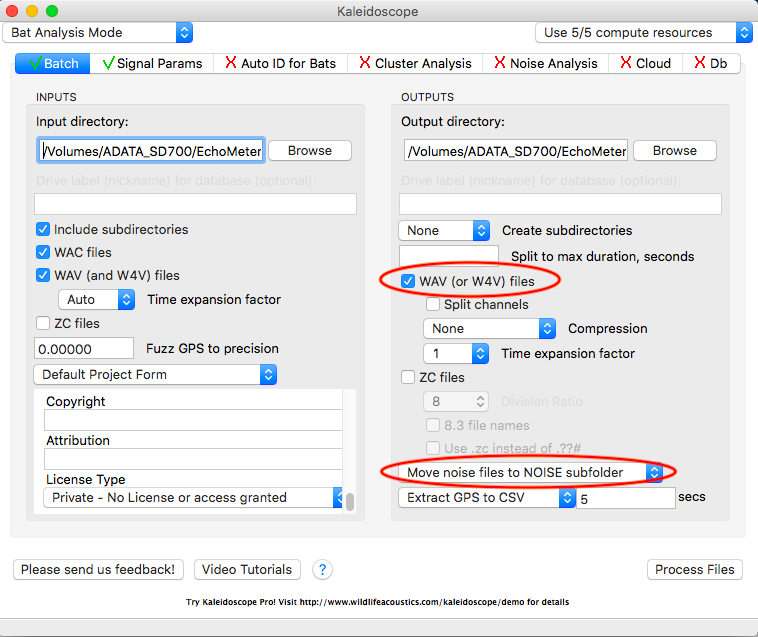
\includegraphics[width=.7\textwidth]{Fig/Batch_proc_for_noise_detection}
\caption{Necessary setting to allow noise detection with the free version of Kaleidoscope.}
\label{Batch_proc_for_noise_detection}
\end{center}
\end{figure}

The following command (one line) inserts the word "Noise" into the AUTO ID column of \texttt{meta.csv} if the recording has been detected as noise:

\begin{lstlisting}
perl -F, -lane 'if($.==1){print}else{
($file = $F[2]) =~ s/^(.*)\.(.*)/$1_000.$2/; 
$file = "NOISE/" . $file; 
if(-e $file){$F[17] = "Noise"}; 
print join(",", @F)
}' meta.csv > meta_with_noise_in_Auto_ID.csv
\end{lstlisting}

Note that on line 2 in the command, the file name taken from \texttt{meta.csv} has to be modified: the string "\_000" has to be inserted. The copied files in the output directory of batch processing have this additional string, but \texttt{meta.csv} contains the names of the source files. The command checks whether a recording file has been put into the subfolder NOISE.

I have used the following settings for noise detection (set in the "Signal Params" tab):
\begin{itemize}
\item minimum frequency of 15 kHz for signals
\item minimum of 2 ms and maximum of 100 ms for the duration of individual pulses
\item maximum of 300 ms for the gap between pulses
\item minimum number of 3 pulses per recording
\end{itemize}

These settings can be found in the output folder in the file \texttt{settings.ini} under section \texttt{[analysis]}. They are not the standard ones and my need to be adjusted based on the distribution of signal parameters from different species.

I have visually checked the 84 recordings that have been detected as noise by Kaleidoscope with these settings. Six of these recordings \emph{did} contain bat calls, either faint or among loud cricket calls (fig. \ref{NoID_20200723_005253}).

\begin{figure}[htbp]
\begin{center}
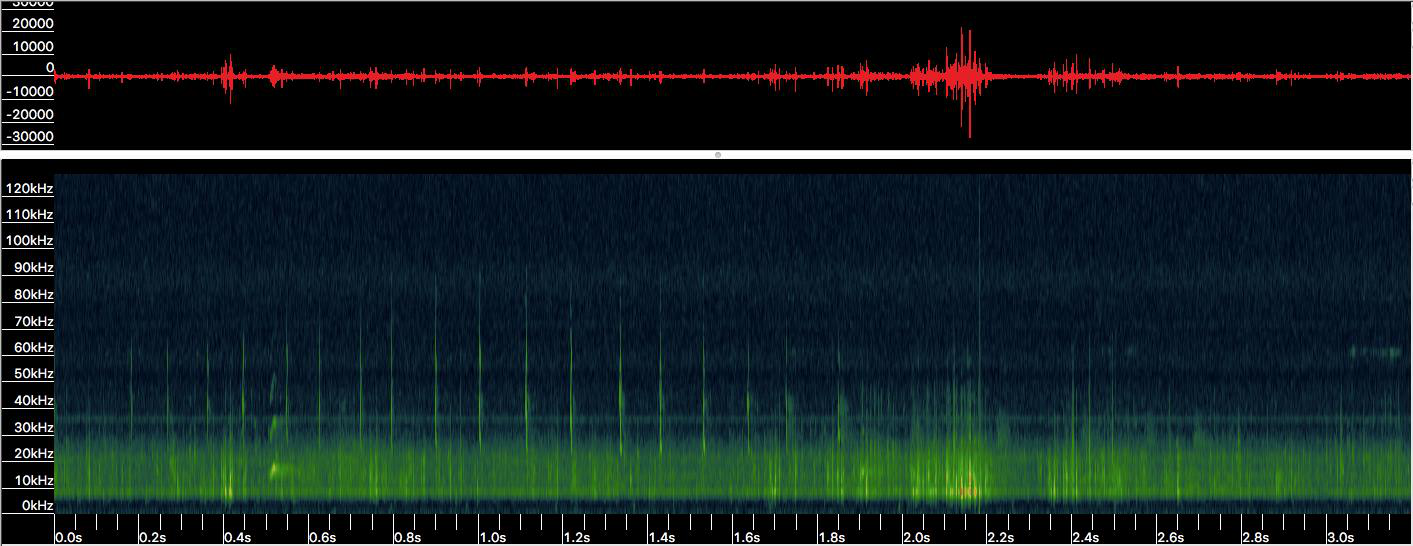
\includegraphics[width=.9\textwidth]{Fig/NoID_20200723_005253}\vspace{2em}
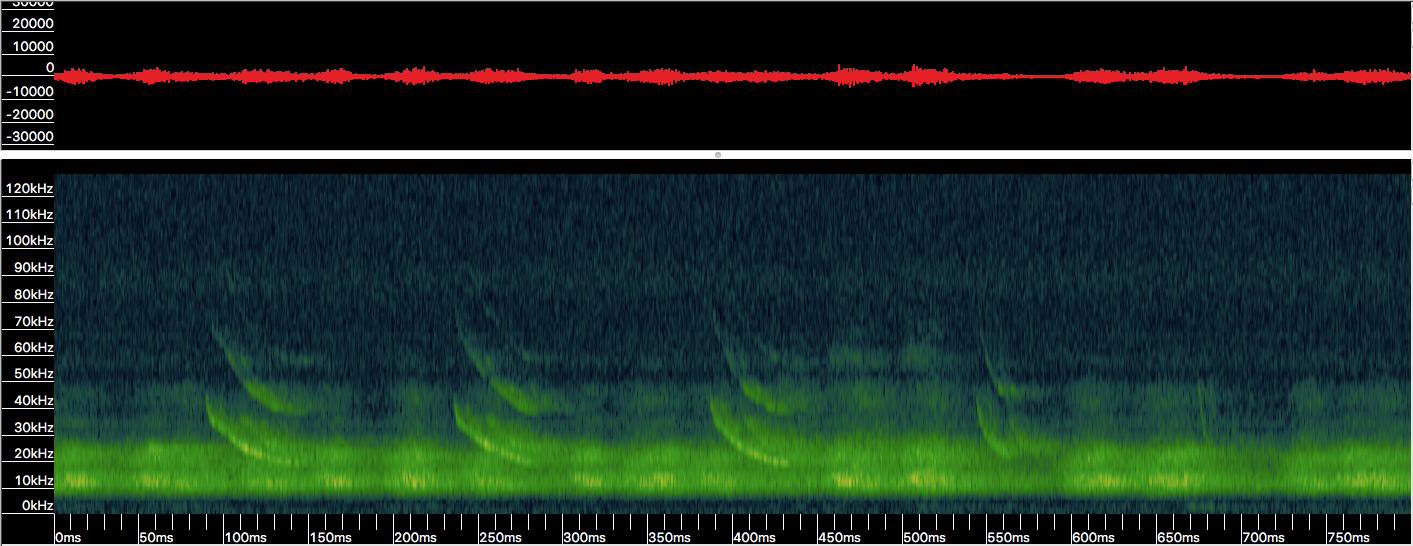
\includegraphics[width=.9\textwidth]{Fig/NoID_20200723_003513}
\caption{Recordings that have been detected as noise. Top: Recording \texttt{NoID\_20200723\_005253} contains faint calls from a \textit{Myotis} species. Bottom: Recording \texttt{NoID\_20200723\_003513} contains bat calls on a background of loud cricket calls.}
\label{NoID_20200723_005253}
\end{center}
\end{figure}

%
%
%
\subsection{How to add more than one species label per recording file}
%
%
%
Under \fbox{Kaleidoscope Help} $\rightarrow$ \fbox{Reference Guide} $\rightarrow$ \fbox{Metadata Panel} one can find the following info:

\begin{quote}
To assign multiple manual IDs, hold the Control key down while pressing one of the user-defined buttons (or the corresponding shortcut key). This will add the label to the Manual ID field, separating multiple entries with commas while also disabling the Auto next file button. 
\end{quote}

On a Mac press the \fbox{cmd} key instead of the \fbox{ctrl} key. The choice of a comma to separate species labels is unfortunate since \texttt{meta.csv} is comma separated. I would therefore recommend to edit multi-species labels so that they are separated by a semicolon.

Usually, when you save \texttt{meta.csv} with \emph{K} it will add double quotes around each field entry, which disrupts further command line manipulation of this important file. Unless you have multi-species labels that are separated by a comma instead of a semicolon, it is save to remove these double quotes again:

\begin{lstlisting}[numbers=none]
tr -d '"' < meta.csv > meta_noquotmark.csv
\end{lstlisting}



%
%
%
\subsection{How to add notes}
%
%
%

In the Metadata panel there is a field called notes. Under \fbox{Kaleidoscope Help} $\rightarrow$ \fbox{Reference Guide} $\rightarrow$ \fbox{Metadata Panel} it says:
\begin{quote}
Under Notes there is an \emph{editable} field which contains field notes and GUANO format metadata if present.
\end{quote}
I have tried to edit this field with the free version of \emph{K}, but it is not saved. It may be that only during batch processing, information that pertains to the whole session of recordings can be saved here. Notes for individual recordings cannot be saved here, at least with the free version of \emph{K}.

A workaround, although more error prone than editing directly in the results window of \emph{K} Viewer, is to create an \texttt{id\_notes.csv} file that contains a selection of columns from \texttt{meta.csv} and then open that file in a spreadsheet application for editing together with \emph{K} Viewer. Since \texttt{meta.csv} already contains a NOTES column, I suggest naming the new notes column "ID NOTES".

The following command will display a numbered list of column headers from \texttt{meta.csv}. 

\begin{lstlisting}[numbers=none]
head -1 meta.csv  | tr ',' '\n' | nl

     1	INDIR
     2	FOLDER
     3	IN FILE
     4	DURATION
     5	DATE
     6	TIME
     7	HOUR
     8	DATE-12
     9	TIME-12
    10	HOUR-12
    11	LATITUDE
    12	LONGITUDE
    13	MODEL
    14	SERIAL NO
    15	FIRMWARE
    16	PREFIX
    17	NOTES
    18	AUTO ID
    19	PULSES
    20	MATCHING
    21	MATCH RATIO
    22	MARGIN
    23	FILES
    24	MANUAL ID
    25	ORGID
    26	USERID
    27	REVIEW ORGID
    28	REVIEW USERID
    29	INPATHMD5
    30	NR
\end{lstlisting}

I then use the following command to create a copy of \texttt{meta.csv} with a selection of columns
\begin{lstlisting}[numbers=none]
cut -d, -f3,5-6,18,24,30 meta.csv > id_notes.csv
\end{lstlisting}

The new "ID NOTES" column can be added to \texttt{id\_notes.csv} in the spreadsheet application. With it \texttt{id\_notes.csv} will have 7 columns. The file format needs to stay the same.

%
%
%
\section{Post-processing \texttt{meta.csv}}
%
%
%

%
%
\subsection{How to join ID NOTES to \texttt{meta.csv}}
%
%

After manual review of recordings in \emph{K} Viewer and adding corresponding notes to \texttt{id\_notes.csv}, the "ID NOTES" column (here the seventh column) can be joined back to \texttt{meta.csv} with the following command line (one line):

\begin{lstlisting}
join -t, -1 3 -2 1  meta.csv <(cut -d, -f1,7 id_notes.csv) 
| tr -d '\r' > meta_with_id_notes.csv
\end{lstlisting}


%
%
\subsection{How to create a KML file from the \texttt{meta.csv} file after manual id}
%
%

The EMT app creates a KML file for each recording session. It would be nice to create an updated KML file after manual review of the recordings. This is what the programme \texttt{style2kml.pl} does. It takes a \texttt{meta.csv} (usually after reviewing the recordings and filling the MANUAL ID column) as well as a(ny) Session*kml file created by the EMT app and creates a KML that contains Placemarks that show the manual id (not the auto id from the EMT app) and the remaining info in \texttt{meta.csv} in a pop-up table in Google Earth. Note, that the programme relies on the \texttt{ogr2ogr} utility from \href{https://gdal.org/download.html}{GDAL}.

\begin{lstlisting}[language=Perl, backgroundcolor = \color{OliveGreen}, basicstyle=\small\ttfamily\color{white}, keywordstyle=\color{YellowOrange}\bfseries,
identifierstyle=\color{Cyan}\bfseries, stringstyle=\color{BrickRed}, commentstyle=\color{blue}, title=\texttt{style2kml.pl}, numbers=left, numberstyle=\color{black}]
use strict;
use warnings;

my $usage = "

usage: $0 --meta <your meta.csv> --EMT_kml <kml from EMT app>

--meta your meta.csv file name (and path)
--EMT_kml any Session*kml file name from EMT app 
[--species species abbreviation as used by Kaleidoscope, e.g. HYPSAV]

prints result to STDOUT
\n";

system("which ogr2ogr > /dev/null") == 0 or 
die "You need to have the utility ogr2ogr installed and in your PATH.
https://gdal.org/download.html\n";

my ($meta, $EMT_kml);
my $species = ""; 

# does what it says in the name
sub parse_command_line {
    while(@ARGV){
        $_ = shift @ARGV;
        if(/^-{1,2}meta$/){$meta = shift @ARGV;}
        elsif(/^-{1,2}species$/){$species = shift @ARGV;}
        elsif(/^--EMT-kml$/){$EMT_kml = shift @ARGV;}
        elsif(/^-{1,2}h(elp)?$/){die $usage;}
    }   
}

parse_command_line();
die $usage unless (defined($meta) && defined($EMT_kml));

# extracts the style definition from a session kml produced by EMT app
# we want to reuse the style in our new KML file
sub get_style{
    my $style_fh;
    open($style_fh, "<", $EMT_kml) or die $!; 
    while(<$style_fh>){
        print if /<Style/ .. /<\/Style>/;
    }   
}


# generate KML from the meta.csv file after manual id
my $cmd = sprintf("ogr2ogr -f KML meta_raw.kml %s -a_srs \'EPSG:4326\' 
-oo X_POSSIBLE_NAMES=LON\* -oo Y_POSSIBLE_NAMES=LAT\* -oo KEEP_GEOM_COLUMNS=NO 
-where  \"\\\"MANUAL ID\\\" LIKE \'%%%s%%\'\" ", $meta, $species);
system($cmd) == 0 or die $?;


# open the KML to which the style should be added
open (my $metaKML, "meta_raw.kml") or die $?;
my ($manual_id, $date, $time);

# add required style info
# use MANUAL ID for marker style (the Session KML uses AUTO ID)
# add date and time in name tag (for chronological sorting in Google Earth)
while(<$metaKML>){
    print;
    # add the style definition after the Document XML tag
    if(/<Document.*>/){
        print get_style();
        #       print "\n";
    }
    # add marker style XML tag to each Placemark
    elsif(/MANUAL ID/ and /SimpleData/){
        ($manual_id) = $_ =~ />(.*)</;
    }elsif(/"DATE">/ and /SimpleData/){
        ($date) = $_ =~ />(.*)</;
    }elsif(/"TIME">/ and /SimpleData/){
        ($time) = $_ =~ />(.*)</;
    }elsif(/<\/ExtendedData>/){
        print "\t<styleUrl>#MarkerStyle", $manual_id, "</styleUrl>\n";
        print "\t<name>", $date, ", ", $time, "</name>\n";
    }
}

# clean up
system("rm -f meta_raw.kml") == 0 or die $!;
\end{lstlisting}

%
%
%
\section{Bat id}
%
%
%
What does the bat id do if there are calls of more than one species in the recording?


%
%
%
\section{Recordings from other detectors}
%
%
%
Can K handle recordings from other bat detectors, like Batlogger?


%
%
%
\section{Miscellaneous}
%
%
%
I have run K with \texttt{Auto ID for Bats} set to \texttt{balanced (neutral)}. The input recordings came from EMT that had already done an auto id on them but with the \texttt{more accurate (conservative)} setting. In the \texttt{id.csv} file the bat id from the EMT app seems to have been copied to the \texttt{Manual ID} column. Twenty-four out of 179 ID's have changed in this process (about one in 7 id's). The auto id in K has changed id's of 9 recordings from a species to \texttt{NoID}, which is strange, since the auto id in K should have been less conservative, i.e. more willing to assign an id. In the other direction K has changed the id of 8 recordings from \texttt{NoID} to a species, i.e. what I would expect to happen occasionally. K has given the new id \texttt{Noise}, which does not occur among the EMT app id's, to 7 recordings. 

The file log.txt indicates that there has been an error reading 4 of the input files. I have tried to open these files with Kaleidoscope individually, but got an error again. I have also tried to find these files in the EMT app on my smartphone, but couldn't find them. I could also not open them with the
program Audacity, while I could open another file with it.

%
%
%
\section{Feature Request}
%
%
%
When working on a small screen (laptop) it would be nice to have the Viewer window, the Results window (table) and the Settings window overlap each other or in full screen size. Then switching between those windows is currently cumbersome (on Mac: F10, then select the window to switch to, Enter). It would be better to have a shortcut for each window, like \texttt{Cmd-1} for the Viewer, \texttt{Cmd-2} for the Results and \texttt{Cmd-3} for the Settings window, for instance.



% 
%\begin{enumerate}
%\item Implement a new random genetic marker technique called \textit{sRAD}.
%\item Find loci linked to Dobzhansky-Muller incompatibilities responsible for  sterility in F$_{1}$ male hybrids of two grasshopper subspecies.
%\end{enumerate}
%
%\begin{itemize}
%\item How many genes are responsible for the observed hybrid male sterility? 
%\item Are these genes disproportionately located on the X-chromosome?
%\end{itemize}
%
%
%\subsubsection{Background}
%Two subspecies of \emph{Chorthippus parallelus} -- \emph{Chorthippus parallelus parallelus} and \emph{C. p. erythropus} -- form a hybrid zone in the Pyrenees. F$_{1}$ male hybrids between \emph{C. p. parallelus} and \emph{C. p. erythropus} from outside the hybrid zone are almost completely sterile with degenerate testes and a severely disrupted meiosis \citep{Hewitt1987}
%$\sim$1800 RAD tags 
% \textsterling1,100.
%(see section \ref{QTL cross} on p. \pageref{QTL cross}),
%\citep[p. 284-319]{CoyneOrr2004}, such as: 
%
%
%\begin{figure*}[htb]%a picture has to be inserted into a figure environment in order to make it floatable; a star at figure has to be added for a two column layout
%\begin{center}
%\subfigure[Oscillogramm (bottom) and traces of the corresponding hindleg movements (top) of a singing \emph{C. montanus} male. Three syllables are shown. (from \citealp{Helversen1994}, p. 271) ]{\label{montanus}\includegraphics[scale=1.0]{montanus}}
%\hfill %pushes the graphics to the left and right margins
%\subfigure[Syllable duration over body temperature in \emph{C. parallelus} (syn. \emph{longicornis}) and \emph{C. montanus} males. (from \citealp{Helversen1987}, p. 121)]{\label{syllable}\includegraphics[scale=1.2]{syllableDuration}}
%\end{center}
%\caption{The songs of \emph{C. montanus} and \emph{C. parallelus} differ only in the duration of their syllables.}
%\label{songdiff}%the label command has to occur after the caption but inside the figure environment to refer (with \ref) to the figure and not the section of the document
%\end{figure*}
%
%
%
%%%% sRAD sketch from Floragenex website
%\begin{figure*}[tbp]
%\begin{center}
%\includegraphics[scale=.25]{RADprocessOverview}
%\caption{\emph{sRAD} is basically Solexa/illumina sequencing of restriction fragment ends. Each restriction site defines the position of two tightly linked RAD tags.} 
%\label{Floragenex}
%\end{center}
%\end{figure*}
%%%%
%
%\underline{s}equenced \underline{R}estriction \underline{S}ite associated \underline{D}NA.
%
%50\% NERC funding 
%
%
%
%
%
%%%% my own sketch of the sRAD library preparation process
%\begin{figure*}[htbp]
%\begin{center}
%\includegraphics[scale=.6]{sRADprocessSketch}
%\caption{(a) The genome is cut but a restriction endonuclease ~~(b) P1 adapters (blue) containing a different 5base pair long nucleotide sequence (red) for each individual sample are ligated to restriction fragment ends. ~~(c) After pooling the P1 ligated samples, they are sheared to below 1kb before a size range is selected on the gel. The shearing step makes the marker technique repeatable. ~~(d) A few steps further, the P2 adapter, a divergent Y adapter, is ligated onto all fragments. In the following PCR, only fragments with at least one P1 adapter will be amplified. ~~(e) Further complexity reduction by restricting the library with frequent cutter restriction enzymes. ~~(f) Solexa sequencing. The first 5 base pairs in the reads identify the individual. A T/A single nucleotide polymorphism is marked by the red frames.} 
%\label{sRADsketch}
%\end{center}
%\end{figure*}
%%%%
%
%
%\begin{quotation}
%``\ldots the most important determinant of [QTL analysis] power is F2 and/or backcross sample size \ldots  small samples sizes lead to systematic overestimation of QTL addititive effects, the so-called \textsc{beavis} effect \ldots simulations suggest that this effect becomes small as experimental sample sizes near $\sim$500 genotyped and phenotyped individuals.'' \citep{Orr2001a} 
%\end{quotation}
%
%The temperature curve in the CT room where the grasshoppers have been recorded is oscillating by 2$^{\circ}$C 
%
%
%
%%%%%%%% PCA table
%% Requires the booktabs package if the memoir class is not being used
%\begin{table}[!htbp]
%\begin{center}
%\topcaption{correlation of peaks with PCA scores} % requires the 'topcapt' package
%\begin{tabular}{@{}lcr@{}}
%\toprule
%& \multicolumn{2}{c}{scaling by:}\\
%& Peak & Individual\\
%\cmidrule(l){2-3} % Partial rule. (r) trims the line a little bit on the right; (l) & (lr) also possible
%& Comp.1 & Comp.1\\
%\midrule
%Peak.1  & -0.8809&-0.8237\\
%Peak.2  & -0.8249&-0.8490\\
%Peak.3  & -0.7623&-0.8563\\
%Peak.4  & -0.8255&-0.6677\\
%Peak.5 & -0.8886&-0.5243\\
%Peak.6  &-0.4218&0.3017\\
%Peak.7  &-0.8427&0.1139\\
%Peak.8  &-0.6538&0.4732\\
%Peak.9  &-0.9358&0.3918\\
%Peak.10&-0.7138&-0.3078\\
%Peak.11 &-0.7750&0.1455\\
%Peak.12& -0.8784&-0.4255\\
%Peak.13 &-0.8469&0.1801\\
%Peak.14 &-0.8413&0.5327\\
%Peak.15 &-0.8619&0.5204\\
%Peak.16 &-0.8038&0.4222\\
%Peak.17 &-0.8171&0.2868\\
%Peak.18 &-0.8320&0.4565\\
%Peak.19 &-0.8707&0.6411\\
%Peak.20 &-0.8834&0.6679\\
%Peak.21 &-0.8377&0.6844\\
%Peak.22& -0.8207&0.6334\\
%Peak.23 &-0.7635&0.5860\\
%\bottomrule
%\end{tabular}
%\label{PCcorrPeak}
%\end{center}
%\end{table}
%%%%%%% PCA table
%
%
%
%\begin{table*} % the asterisk puts the table on that page, I don't know why, but here it fits better
%\centering
%\topcaption{MANOVA results for species difference of CHC blends among females using data scaled by peak.} % the top caption needs to be before the begin{tabular} command
%\begin{tabular}{@{}lrrrrrr@{}}
%\toprule
%& \small{Df} & \small{Pillai} & \small{approx F} & \small{num Df} & \small{den Df} & {Pr($>$F)}\\  
%\midrule  
%\small{Species} & \small{1} & \small{0.817}  &   \small{6.19}    & \small{23}    & \small{32} & \small{1.9e-06***}\\
%\small{Residuals}  &   \small{54} & & & & & \\                                       
%\bottomrule
%\end{tabular}
%\label{manova}
%\end{table*}
%
%
%
%%%%% multivariate outlier individuals
%\begin{table}[!htbp]
%\centering
%\topcaption{Multivariate outlier individuals.} % requires the 'topcapt' package
%\begin{tabular}{@{}lr@{}}
%\toprule
%Individual & $\sqrt[2]{Mahanalobis}$\\
%\midrule
%26parF & 7.066\\
%49parF & 7.025\\
%50parF & 5.999\\
%52parF & 7.186\\
%53parF & 5.976\\
%55parF & 6.740\\
%85parF & 6.819\\
%29monF\underline{}Fin & 6.349\\
%32monF\underline{}Fin & 6.059\\
%84monF\underline{}Fin & 6.871\\
%61monF\underline{}Ger & 5.938\\
%\bottomrule
%\end{tabular}
%\label{outlier}
%\end{table}
%
%
%
%\bibliographystyle{apalike}
%\onecolumn
%\setlength{\columnsep}{20pt}
%\begin{multicols}{2} 
%% the separation of the columns has been set in the preambel
%%\begin{multicols}{2}
%
%\bibliography{/Users/Claudius/Documents/MyLiterature/Literature}
%
%\end{multicols}
%
\end{document}
